\documentclass[adobefonts]{ctexart}
%\documentclass[winfonts]{ctexart}

\CTEXoptions[captiondelimiter={\quad}]


\usepackage{amsmath}            % AMS的数学宏包
\usepackage{amssymb}            % AMS的数学符号宏包
\usepackage{graphicx}           % 插入图片需要的宏包
\usepackage{float}              % 强大的浮动环境控制宏包
\usepackage{framed}             % `shaded'环境需要用到
\usepackage{enumitem}           % 增强列表功能
\usepackage{alltt}              % 在`alltt'环境中为等宽字体, 但可以使用LaTeX命令

% \usepackage{shortvrb}           % 简化\verb的写法
% \MakeShortVerb{\|}
\usepackage{listings}
\lstset{language=bash}
\lstset{extendedchars=false}
\lstset{breaklines}
\lstset{stepnumber=2}
\lstset{backgroundcolor=\color{lightgray}}


\usepackage{color}              % 可以定义各种颜色
\usepackage[x11names]{xcolor}   % 下面的RoyalBlue3颜色需要用到的宏包
% 自定义的几种颜色
\definecolor{shadecolor}{gray}{0.85}

% \definecolor{darkblue}{rgb}{52,101,164}
% \definecolor{darkgreen}{rgb}{78,154,6}

% % 设置背景颜色
% \definecolor{bisque}{rgb}{.996,.891,.755}
% \pagecolor{bisque}

\usepackage[pdfauthor={Dreamseeker},
  pdftitle={介绍vim的强大功能},
  colorlinks=true,
  urlcolor=blue,
  linkcolor=RoyalBlue3]{hyperref} % 为超链接设置颜色, 修改PDF文件信息

%\CTEXsetup[name={实验,},number={\chinese{section}}]{section}


\title{\textbf{介绍vim的强大功能}}
\author{deanraccoon@gmail.com}
% \date{}

\usepackage[pagestyles]{titlesec} % 定制页眉页脚
% % 设置页眉页脚
% \newpagestyle{main}{%
%   \sethead[$\cdot$~\thepage~$\cdot$][][\thesection\quad%
%   \sectiontitle]{\thesection\quad\sectiontitle}{}{%
%   $\cdot$~\thepage~$\cdot$}
%   \setfoot{}{}{}\headrule}
% \pagestyle{main}
% \renewpagestyle{plain}{\sethead{}{}{}\setfoot{}{}{}}
\pagestyle{plain}

\usepackage[top=0.75in,bottom=0.5in,left=1in,right=1in]{geometry} % 设置页边距

\setlength{\belowcaptionskip}{1em} % 设置caption之后的距离

% For LaN
\newcommand{\LaN}{L{\scriptsize\hspace{-0.47em}\raisebox{0.23em}{A}}\hspace{-0.1em}N}
\begin{document}

\maketitle
\tableofcontents
\newpage

\section{vim的乱码问题}
在很少的情况下,vim也会出现乱码,不用去抱怨vim的配置复杂,只要明白各个配置的含义,就可以逸劳永逸的解决它

关于编码,一共是这4个
\begin{itemize}
\item encoding 

设置vim的内部编码,与文件的具体编码也没有关系。通常是改成utf-8就不用再动了

\item termencoding 

在命令行模式的情况下,设置编码,\textbf{一定要与term的编码一致},比如term是utf-8,那么termencoding也应该是utf-8.同样如果term是GBK编码,那termencoding也要是GBK编码. 这个问题通常会在远程登录时出现,比如putty和securyCRT都可以改自己的编码,主要要和termencoding一致. 如果是用gvim的话,这个参数不起作用

\item fileencoding  

有2个用途。1,配置新建一个文件时,文件的默认编码。 2.打开一个已有的文件,通过设置一个与源文件编码不同的fileencoding,再保存。达到iconv的效果。一般情况下fileencoding最好和本地的locale一致. 我以前犯一个错误,发现文件乱码时,用fileencoding修改成别的编码,再保存。这样就把文件越改越乱了。

\item fileencodings

打开的文件会不会乱码,主要靠这个设置了!vim根据fileencodings的顺序判断文件的编码,当encoding设置成utf-8时,默认的顺序是ucs-bom,utf-8,default,latin1,其中"default"表示当前locale的配置. 可以看出这个默认的设置有点儿问题。当default是latin1的时候,而你的文件又是GBK编码的方式,那么就会显示乱码了。如果只对中文而言改成ucs-bom,utf-8,gbk就可以了。删去default,在
这种情况下,即使locale是8859-15也不会影响中文. 缺点是如果文件是8859-15编码的话,那打开就成乱码了。因为GBK不和8859-15兼容。所以最完整的解决方案还是在所有的地方都使用utf-8编码,就没有问题了
\end{itemize}
总的来说打开文件能不能正确显示中文,就只需要了检查encoding, fileencodings, termencoding(fileencoding与打开文件时无关, 只说明保存文件时的编码)。检查可以分3步。

1. encoding只要设置成utf-8就不用管了。与乱码无关

2. 保证termencoding与term的编码一致,并且都支持中文,比如utf-8,GBK,utf-16

3. 检查fileencodings的编码顺序。一般要求是先ucs-bom,utf-8 然后其他可能的编码,比如GBK。


更加详细推荐vim的帮助,非常详细,我也是看vim的帮助学的。
还有滇狐的文章可以参考



\subsection{场景举例}
\subsubsection{locale编码utf8时}
现在一般新linux都是默认utf8,用locale命令检查一下就可以了

set encoding = utf-8
set termencoding = utf-8
set fileencoding = utf-8
set fileencodings = ucs-bom,utf-8,default,gbk

fileencodings加上gbk,即使文件是gbk编码,也没有问题了.
如果你是ssh上去的,把你的客户端的编码改成utf-8就可以了

\subsubsection{locale编码是GBK}
vim的内部编码encoding不用改变,termencoding与ssh客户端或者xterm的编码一致

set encoding = utf-8
set termencoding = GBK
set fileencoding = GBK
set fileencodings = ucs-bom,utf-8,default,gbk

\subsubsection{locale编码是8859-15}
如果系统的编码不兼容GBK.怎么办?比如搞出个8859-15来。
如果只是自己用的话,当然是改成utf-8! 只要把export LC\_ALL = zh\_CN.utf8,就ok了
如果必须这样的话,那显然bash里就不可以输入中文了(因为bash认为编码是8859-1, 如果还可以敲入中文,但是删除的总是半个汉字,说明
你的term还是支持中文的,bash已经不支持了). 在这种情况下,只要term还能显示中文,也可以通过设置vim达到编辑中文的功能!

set encoding = utf-8

内部编码始终不用变
set termencoding = utf-8

term的编码始终要与termencoding一直,但一定要是支持中文的编码,比如gbk,utf8 

set fileencoding = utf-8

如果你要在新文件里输入中文,必须要用支持中文的编码了,如果不需要输入中文,那就改成8859-15,与locale一致.

set fileencodings = ucs-bom,utf-8,gbk

去掉default,因为default是8859-15,会比gbk先匹配到, 并且显示出乱码

在locale不支持的情况下还搞中文,何必对自己这么坏呢?

总的来说只有这些需要注意的地方,vim的3个选项和term的编码。可能有时候你会发现在bash里无法输入中文,或者删除中文的时候只删除半个汉字,那是因为
1.本地的locale与你的term的编码不一致。 或者 2. locale编码和term一样了,但是编码却不支持中文。只要注意这2个问题,bash中
的乱码也好解决.

\section{vim的奇巧淫技}
使用vim这个编辑器也很长时间了,从最初不知道怎么退出,到后来自己修改插件,但是仍然发现
有很多强大的功能没有用到,vim的基本用法已经介绍的够多了的,不需赘述,各种插件也各具特色,
本文介绍一些容易忽略的vim强大的功能,抛砖引玉
\subsection{强大的text object}
用:h object可以看到text object的帮助,帮助中的第一句话非常重要
说明textobject是在visual mode里用到的。

什么是visual mode?\\
在普通模式下按v,在状态栏显示出\textbf{可视},表示进入了visual mode,当然
如果是英文版,状态栏就显示出\textbf{visual}.

引号中的文字,一个函数的所有内容,用text object的方式,可以飞快
地选择到,举个例子说明,看下图,要一次选中section的标题:vim的奇巧淫技,
见下图

\begin{figure}[htbp]
	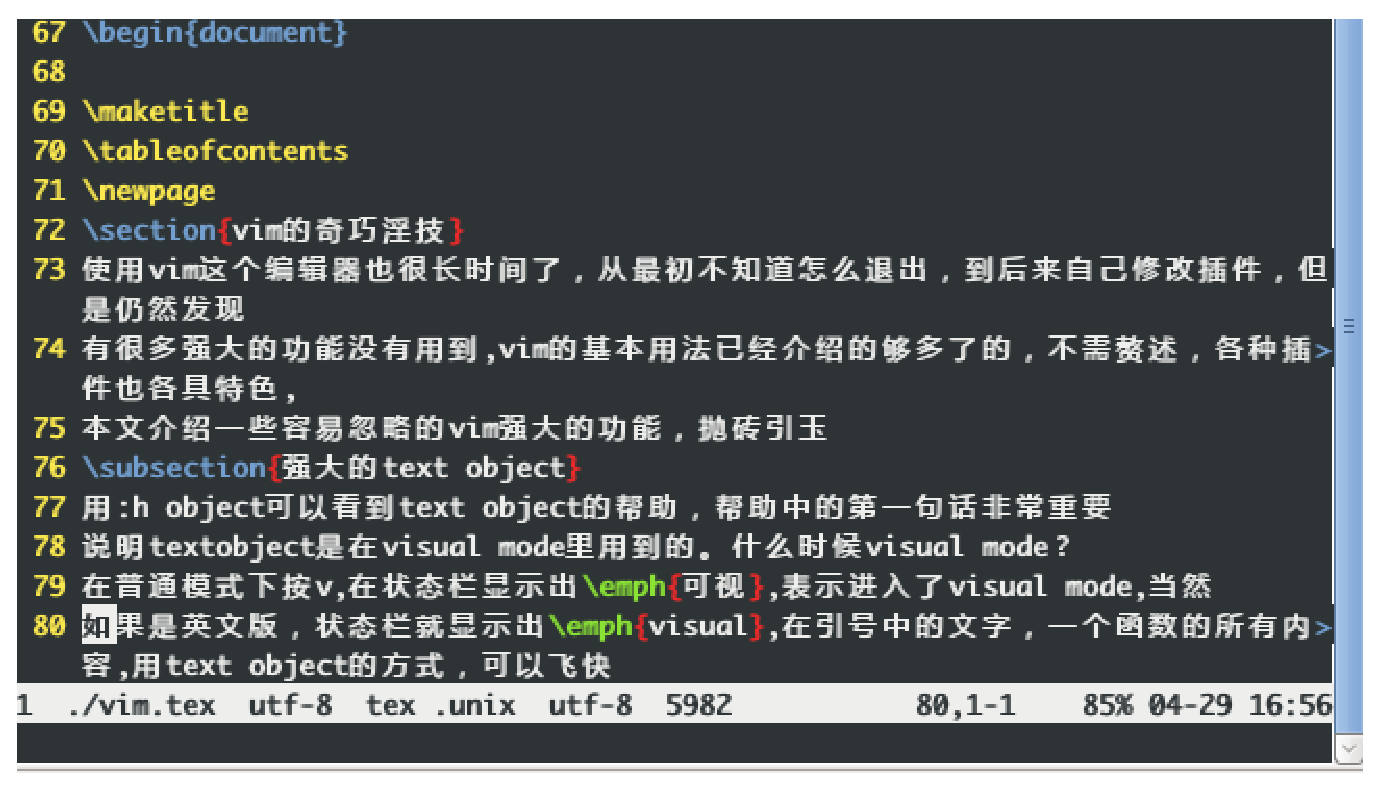
\includegraphics[width=12cm]{select.eps}
\end{figure}
在normal模式下,光标移动到大括号的里面任意位置,用命令\textbf{vi\{},就会发现,大括号内的内容都高亮了
v表示用visual mode,i表示选择不包括编辑,如果用a就表示包括边界,\{表示边界是大括号.
这三个键按完,就选择了大括号内的所有内容
\begin{figure}
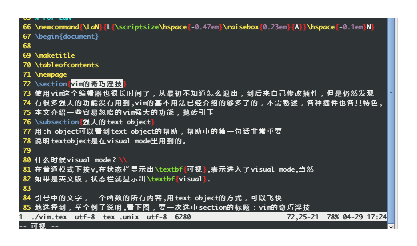
\includegraphics[width=12cm]{selected.eps}
\end{figure}

只要用类似的命令,可以很快的选择一段文字
\begin{itemize}
\item  \textbf{vi"}~~选中引号内文字
\item  \textbf{vi[}~~选中\{\}的文字,在写c文件时很有用
\item  \textbf{vip}~~选中一段文字
\item  \textbf{...}
\end{itemize}
这样的命令有很多,可以自由组合,vim的文档里有完整的列表,请读者自己尝试
\subsection{犀利的列模式}
最早知道列模式是在ultraedit,ultraedit的列模式也是它的一个卖点,强大的vim也有类似的列模式功能

在普通模式下按v会进入普通的visual mode,按\textbf{Ctrl-v}进入列模式的visual mode.
比如我们有这样一个任务,在下面的文件中,在序号后添加hello,这个word
\begin{verbatim}
1.world
2.linux
3.vim
\end{verbatim}
对正则表达式熟悉的同学,自然而然想到只要用一个正则替换就可以完成这个功能,用命令
\begin{verbatim}
%s/\d\./& hello \/g 
\end{verbatim}
但在这里,我还重点介绍采取列模式的方法实现插入hello这个字符串,这个操作也更加直观,
\begin{enumerate}
	\item 移动光标到\textbf{.}处
	\item 按下\textbf{Ctrl-v},进入列模式
	\item 移动光标到最后一行的\textbf{.}处,如下图
\begin{figure}[htbp]

\includegraphics[width=4cm]{col-visual-highlight.eps}
\end{figure}
	\item 按下大写的A,表示在\textbf{.}后插入,如果是大写的I,表示在\textbf{.}前插入
	\item 这样就进入的列模式的插入状态,编辑文本,插入hello, 在编辑的过程中,并不会像ultraedit一样
          在下面实时显示内容,确定一行编辑完成以后,按两下Esc键,可以看到hello,已经自动在后面2行插入了
\end{enumerate}

用列模式也可以很容易删除3行的hello,字符串,用\textbf{Ctrl-v}进入列模式,现在hello,按下\textbf{x},完成删除!



\subsection{巧用书签功能}
用:h m查看vim帮助
书签功能对于文本编辑器的重要性不言而喻,简单的说就是


\begin{tabular}{|c|c|c|}
\hline
:marks & 显示所有书签 & 数字0-9和字符[,自动填入的,有不同的 意义\\ \hline
m[a-z] & 设置临时书签 & 只在当前文件可用 \\ \hline
m[A-Z] & 设置永久书签 &  与传统的书签的功能相同\\ \hline
跳转标签 & '{a-zA-Z0-9}   &   注意\textbf{'}是单引号   \\ \hline
\end{tabular}


传统的书签功能就不说了,重点介绍临时书签的功能。

\begin{tabular}{c c}
'0  &  可以跳转到最后编辑的文件               \\
'.  &  跳转到当前文件最后编辑的地方           \\
''  &  跳转到最后一次跳转之前的位置           \\
...
\end{tabular}

比如编辑一个很长的文件,需要在一段文字间做一次替换,可以在这段文字头ma,做一个书签
在文字尾,开始敲入命令,把所有emacs字符替换成vim
\begin{verbatim}
:'a,. s/emacs/vim/g 
\end{verbatim}

其中\textbf{.}表示当前行,灵活使用书签,能大大提高编辑效率

\subsection{全面的剪贴板}
\subsection{缩进的故事}

\input{../readme}
\end{document}
